% ---------------------------------------------------------------------------
%  BrainFlow -- progress report for supervision
%  Compile:  pdflatex progress_report.tex  (twice, for cross-references)
%  Requires: amsmath, amssymb, booktabs, geometry, hyperref, tikz, xcolor
% ---------------------------------------------------------------------------
\documentclass[11pt,a4paper]{article}

\usepackage[T1]{fontenc}      % lmodern + T1: scalable fonts, required by microtype
\usepackage{lmodern}
\usepackage[margin=2.4cm]{geometry}
\usepackage{amsmath,amssymb,amsthm}
\usepackage{booktabs}
\usepackage{xcolor}
\usepackage{tikz}
\usetikzlibrary{arrows.meta,positioning,fit,backgrounds}
\usepackage[colorlinks=true,linkcolor=blue!55!black,citecolor=blue!55!black,
            urlcolor=blue!55!black]{hyperref}
\usepackage{microtype}

\newcommand{\Sph}[1]{\mathbb{S}^{#1}}
\newcommand{\Exp}{\operatorname{Exp}}
\newcommand{\Log}{\operatorname{Log}}
\newcommand{\Proj}{\mathcal{P}}
\newcommand{\Tang}[1]{T_{#1}}
\newcommand{\R}{\mathbb{R}}
\newcommand{\E}{\mathbb{E}}
\newcommand{\gt}{\mathrm{gt}}

\theoremstyle{definition}
\newtheorem{observation}{Observation}
\newtheorem{remark}{Remark}

\title{\textbf{BrainFlow}\\[2mm]
\large A Riemannian flow-matching prior over CLIP token sequences\\
for fMRI-to-image reconstruction\\[4mm]
\normalsize Design evolution, mathematical challenges, and current standing}
\author{Progress report for supervision}
\date{13 August 2026}

\begin{document}
\maketitle

\begin{abstract}
\noindent
This report documents the development of \textbf{BrainFlow}, a system that
reconstructs viewed images from fMRI recordings in the Natural Scenes Dataset
(NSD). The scientific contribution is not the reconstruction pipeline --- whose
outer stages follow MindEye2~\cite{scotti2024mindeye2} --- but the
\emph{prior}: the generative model that maps brain activity to the
$256\times1664$ ViT-bigG token sequence consumed by a frozen unCLIP decoder. We
model that sequence on the \emph{oblique manifold} $(\Sph{d-1})^{N}$, a product
of spheres over the token directions, and learn a Riemannian flow-matching
transport on it.

The report is organised as a chronology, because the design was not planned in
advance: each stage was forced by a measurement from the previous one. We give
particular attention to the mathematical and geometric obstacles that arose ---
the choice of representation, the singularities of the geodesic interpolant, the
conditioning of the flow-matching objective, and the commensurability of loss
terms with different natural scales --- and to how each was resolved. We close
with an argument, both empirical and theoretical, that \textbf{PixCorr is not a
sound optimisation target} for this class of model, and that ranking statistics
should be preferred.
\end{abstract}

\tableofcontents

% ===========================================================================
\section{Problem setting}
% ===========================================================================

\subsection{Task and data}

Given a single fMRI volume $y \in \R^{V}$ recorded while a subject viewed an
image $x$, reconstruct $x$. We use the Natural Scenes
Dataset~\cite{allen2022nsd}, 7T, $1.8$\,mm, restricted to the
\texttt{nsdgeneral} ROI ($V \approx 13$--$16{,}000$ voxels depending on
subject), on subjects 1, 2, 5 and 7. Training uses roughly $27{,}000$ trials per
subject; evaluation uses the $982$ held-out images that all subjects saw, with
the three repeated presentations averaged in voxel space before encoding.

The scale of the data is the single most important fact about this project:
$\sim\!27$k training pairs is very little for a model in the hundreds of
millions of parameters, and essentially every design decision below is
downstream of that constraint.

\subsection{Pipeline}

\begin{center}
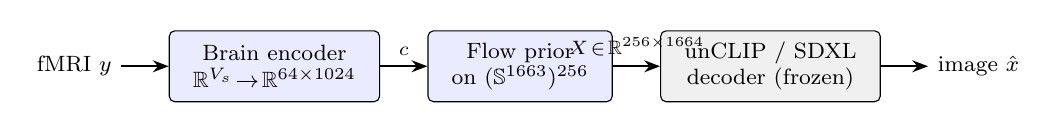
\begin{tikzpicture}[
  node distance=6mm,
  box/.style={draw, rounded corners=2pt, minimum height=9mm, align=center,
              inner xsep=3mm, font=\footnotesize},
  frozen/.style={box, fill=black!6},
  learn/.style={box, fill=blue!8},
  ar/.style={-{Stealth[length=2mm]}, thick}
]
\node[learn] (enc) {Brain encoder\\$\R^{V_s}\!\to\!\R^{64\times1024}$};
\node[learn, right=of enc] (prior) {Flow prior\\on $(\Sph{1663})^{256}$};
\node[frozen, right=of prior] (dec) {unCLIP / SDXL\\decoder (frozen)};
\node[left=of enc, font=\footnotesize] (in) {fMRI $y$};
\node[right=of dec, font=\footnotesize] (out) {image $\hat{x}$};
\draw[ar] (in) -- (enc);
\draw[ar] (enc) -- node[above, font=\scriptsize] {$c$} (prior);
\draw[ar] (prior) -- node[above, font=\scriptsize] {$X\!\in\!\R^{256\times1664}$} (dec);
\draw[ar] (dec) -- (out);
\end{tikzpicture}
\end{center}

The decoder is frozen throughout. Everything the model can express must
therefore be expressed in the token sequence $X$, which makes the geometry of
that sequence the central modelling question.

% ===========================================================================
\section{Chronology of the design}
% ===========================================================================

\subsection{Stage A (June 2026): flow matching in VAE latent space}

The first architecture was a conditional flow-matching (CFM) model
\cite{lipman2023flow,liu2023rectified} over Stable-Diffusion VAE latents, with a
UNet velocity field conditioned on brain tokens and an InfoNCE alignment term.
We explored perceptual (LPIPS) and $L_1$ pixel auxiliaries, token counts from
16 to 64, and a variant in which the flow source was derived from the
conditioning rather than from noise.

The decisive negative result came from that last variant. Training loss fell
from $0.70$ to $0.095$ over five epochs while reconstruction quality
\emph{fell}. The mechanism was instructive and recurs later in this report: when
the source of the flow is a learned function of the conditioning, and gradients
are allowed to flow into it, the model can drive the source onto the target,
making the velocity identically zero. The objective is then satisfied by a
degenerate solution that transports nothing.

\begin{observation}[recurring]\label{obs:degenerate}
In a flow-matching model whose source distribution is learned, the objective
alone does not identify a useful transport. One must either (i) prevent the
source from collapsing onto the target, or (ii) ensure the source retains
genuine dispersion. We use both devices in Stage E.
\end{observation}

Stage A plateaued around PixCorr $0.12$--$0.15$. The diagnosis was that
predicting VAE latents directly asks the model to produce high-frequency
information that fMRI does not contain.

\subsection{Stage B (June 2026): predicting CLIP tokens, not pixels}

We restructured around the MindEye2 spine: predict the $256\times1664$
penultimate ViT-bigG token sequence and hand it to a frozen unCLIP decoder. This
moves the learning problem into a semantic space where fMRI does carry signal,
and removes image synthesis from the training loop entirely.

This stage established the single-subject baseline of CLIP-2way $\approx 0.82$
that we still measure ourselves against, and it exposed the representational
question that became the project's contribution.

\subsection{Stage C (late June 2026): the geometry of the token sequence}
\label{sec:stageC}

The bigG token sequence is \emph{not} unit-normalised: each token
$X_i \in \R^{1664}$ has its own magnitude, and the decoder consumes the raw
values. Two obvious options both fail:

\begin{itemize}
\item Model $X$ as a flat Gaussian in $\R^{256 \times 1664}$ (standardised
      Euclidean CFM). This ignores that the semantic content of a CLIP token is
      carried by its \emph{direction} --- every downstream CLIP metric is a
      cosine --- and it lets the flow wander off the thin shell where real
      tokens live.
\item $L_2$-normalise the sequence and model it on a sphere. This destroys the
      magnitudes the decoder needs, and there is no way to recover them.
\end{itemize}

\paragraph{Resolution: a polar reparametrisation.}
We split each token about a fixed mean $\mu$,
\begin{equation}\label{eq:polar}
X_i \;=\; \mu \;+\; r_i\, z_i,
\qquad r_i = \lVert X_i - \mu\rVert \in \R_{+},
\qquad z_i = \frac{X_i-\mu}{r_i} \in \Sph{d-1},
\end{equation}
with $d = 1664$. The map is a bijection, hence lossless: the decoder still
receives exact raw tokens. The \emph{directions} $z = (z_1,\dots,z_N)$ live on
the product of spheres
\begin{equation}
\mathcal{M} \;=\; (\Sph{d-1})^{N},\qquad N=256,
\end{equation}
known as the \emph{oblique manifold}, and are modelled by a Riemannian flow
matching prior~\cite{chen2024riemannian}. The \emph{radii} $r$ are handled by a
lightweight side model.

This is an \emph{imposed} reparametrisation, not native geometry --- a point
raised in supervision and worth stating plainly. Its justification is empirical
and is given in \S\ref{sec:diagnostic}.

\paragraph{A structured two-head factorisation.}
The pooled CLIP embedding $c_{\mathrm{cls}} \in \Sph{1279}$ is a near-complete
semantic summary of the image. We therefore factor
\begin{equation}
p(X \mid c) \;=\; \underbrace{p(c_{\mathrm{cls}} \mid c)}_{\text{global head, RCFM on }\Sph{1279}}
\;\cdot\;
\underbrace{p(X \mid c,\, c_{\mathrm{cls}})}_{\text{patch head, RCFM on }\mathcal{M}},
\end{equation}
sampling the global direction first and conditioning the patch flow on it, so
that global semantics steer local detail.

\subsection{Stage D (July 2026): the low-level pathway --- a clean negative result}
\label{sec:lowlevel}

MindEye2 attains its pixel-level scores by \emph{fusing} a semantic pathway with
a low-level one that predicts a blurry image used to initialise the diffusion
sampler (\texttt{img2img}) rather than starting from noise. We implemented the
same mechanism and, over four successive designs, failed to make it help:

\begin{enumerate}
\item mean-pooled brain tokens $\to$ blurry RGB;
\item a spatial $8\times8$ token grid $\to$ upsampler;
\item a head reading \emph{raw voxels} through its own encoder;
\item the same, with $L_1$ loss and a lower-resolution ($64^2$) target.
\end{enumerate}

Designs 1--3 all plateaued at a blur-MSE of $\approx 0.070$, which we determined
was exactly the score of \emph{predicting the per-image mean colour}. Design 3
carried $17.4$M parameters against design 2's $1.5$M and scored identically
($0.0699$ vs.\ $0.0702$), which established that the head was never the
bottleneck. Design 4 removed the mean-seeking behaviour and promptly overfitted
instead: validation blur-MSE rose monotonically $0.083 \to 0.104$ across 150
epochs.

\begin{observation}
Underfitting and overfitting both failing on the same target is evidence that
the \emph{target} is wrong, not the capacity. A $128^2\!\times\!3 = 49$k-dimensional
RGB image is not a learnable intermediate from $27$k fMRI trials.
\end{observation}

This result matters beyond its own scope: it is the reason our pixel-level
metrics sit far below the published tables, and it motivates the discussion in
\S\ref{sec:pixcorr}. A fifth design predicting the VAE latent
$E(\mathrm{blur}(x)) \in \R^{4\times96\times96}$ --- the quantity the sampler
actually starts from --- is implemented but not yet the subject of a full run.

\subsection{Stage E (August 2026): re-deriving the transport}
\label{sec:stageE}

By late July the picture was unambiguous. The prior was the bottleneck: the
regression anchor achieved a mean token cosine of only $\approx 0.37$, and the
flow prior --- transporting from a uniform source --- did not improve on it.
Widening the encoder from 2048 to 4096 made things worse and overfitted from the
first evaluation, confirming that the model was data-starved rather than
capacity-starved.

Stage E is the response, and is the current state of the work. It consists of
three changes, each derived in \S\ref{sec:math}: an \emph{informative source}
for the flow (\S\ref{sec:source}), an \emph{endpoint parametrisation} of the
velocity field (\S\ref{sec:param}), and a \emph{discriminative term on the
decoder path} (\S\ref{sec:contrastive}).

\begin{table}[t]
\centering
\footnotesize
\begin{tabular}{@{}llp{8.6cm}@{}}
\toprule
\textbf{Date} & \textbf{Stage} & \textbf{Development} \\
\midrule
2026-06-01 & A & CFM over VAE latents; token attention, InfoNCE alignment \\
2026-06-11 & B & Pivot to bigG token targets + frozen unCLIP decoder; multi-subject caches \\
2026-06-20 & B & SoftCLIP contrastive alignment; NaN-stable training \\
2026-06-23 & C & \emph{Decision}: Riemannian flow matching on the oblique manifold is the contribution \\
2026-06-24 & C & Geometry primitives: slerp, geodesic velocity, exp/log maps, polar encode/decode \\
2026-06-29 & C & Two-head factorisation (global $\Sph{1279}$ + patch $\mathcal{M}$); token diagnostic; per-token radius head \\
2026-06-30 & C & First full runs: sphere stable and ahead of the Euclidean baseline, which diverged \\
2026-06-30 & D & Low-level \texttt{img2img} pathway added \\
2026-07-12 & D & Frozen-prior warm start; spatial head; voxel-fed head \\
2026-07-18 & D & $L_1$ loss, lower-resolution target; decode-configuration sweep \\
2026-07-21 & D & Three full runs; low-level pathway concluded as a negative result \\
2026-08-06 & --- & Evaluation-correctness pass; leakage-free selection; BiMixCo \\
2026-08-12 & E & Informative flow source with a variational posterior \\
2026-08-13 & E & Endpoint parametrisation; per-position centring; ranking-based selection \\
\bottomrule
\end{tabular}
\caption{Development timeline. Each stage was initiated by a measurement from
the previous one rather than by a plan.}
\end{table}

% ===========================================================================
\section{Mathematical and geometric challenges}
\label{sec:math}
% ===========================================================================

\subsection{Riemannian flow matching on the oblique manifold}

On the sphere the flow-matching construction of~\cite{lipman2023flow} is
replaced by its geodesic counterpart~\cite{chen2024riemannian}. For endpoints
$z_0, z_1 \in \Sph{d-1}$ separated by $\theta = \arccos\langle z_0,z_1\rangle$,
the conditional path is the great-circle interpolant
\begin{equation}\label{eq:slerp}
z_t \;=\; \frac{\sin\!\big((1-t)\theta\big)}{\sin\theta}\, z_0
       \;+\; \frac{\sin(t\theta)}{\sin\theta}\, z_1 ,
\end{equation}
and the target velocity is its time derivative,
\begin{equation}\label{eq:slerpvel}
u_t \;=\; \frac{\mathrm{d}z_t}{\mathrm{d}t}
       \;=\; \frac{\theta}{\sin\theta}
             \Big(\!-\cos\!\big((1-t)\theta\big) z_0 + \cos(t\theta)\, z_1\Big)
        \;\in\; \Tang{z_t}\Sph{d-1},
        \qquad \lVert u_t\rVert = \theta .
\end{equation}
The network output is projected onto the tangent space,
$\Proj_{z}v = v - \langle z,v\rangle z$, and integration uses the exponential map
$\Exp_z(w) = \cos\lVert w\rVert\, z + \sin\lVert w\rVert\, w/\lVert w\rVert$,
so that iterates remain on the manifold exactly rather than approximately. We
use a geodesic Heun scheme. Because $\mathcal{M}$ is a product, all of this acts
independently per token and broadcasts.

\paragraph{Challenge: removable singularities at both ends of the geodesic.}
Equations \eqref{eq:slerp}--\eqref{eq:slerpvel} carry a $1/\sin\theta$ factor
that is singular both when the endpoints coincide ($\theta \to 0$) and when they
are antipodal ($\theta \to \pi$). Both limits are removable --- as
$\theta \to 0$ the interpolant tends to the normalised chord and the velocity to
$z_1 - z_0$ --- but a naive implementation produces $0/0$ and propagates
\texttt{NaN} through the whole batch. We guard each singular expression on the
measure-zero set where it degenerates and substitute the analytic limit.

A related and subtler issue concerns the logarithmic map
$\Log_z(y) = \theta\, \Proj_z y / \lVert \Proj_z y\rVert$. Writing
$\theta = \arccos\langle z,y\rangle$ requires clamping the argument away from
$\pm 1$ to keep the derivative finite, and that clamp puts a \emph{floor} under
the output: at $y = z$ the map returns a small but non-zero vector in a
numerically arbitrary direction. This is harmless when $\Log$ merely measures a
displacement, but it is fatal in \S\ref{sec:param}, where $\Log_{z_t}(\hat{z}_1)$
is evaluated with $\hat z_1 = z_t$ and the residual accumulates over integration
steps. The stable formulation uses
\begin{equation}
\theta \;=\; \operatorname{atan2}\!\big(\lVert \Proj_z y\rVert,\ \langle z,y\rangle\big),
\end{equation}
which is exact and differentiable at $\theta = 0$ and well-conditioned near
$\theta = \pi$, and needs no clamp at all.

\paragraph{Challenge: the sampler queries the field where it was never trained.}
Training samples $t$ from a logit-normal distribution, which places almost no
mass at the endpoints, yet a naive integrator evaluates $v_\theta$ at exactly
$t=0$ and $t=1$. On a manifold this is worse than in flat space, because an
out-of-distribution velocity does not merely misplace the iterate --- it can
push it into a regime where the retraction is ill-conditioned. We mix a fraction
of uniform $t$ into training and clamp query times to $[t_{\min}, t_{\max}]$.

\paragraph{Guidance.}
Classifier-free guidance must be formed in the tangent space, as
$v = v_{\varnothing} + s\,(v_c - v_{\varnothing})$ followed by re-projection.
We note in \S\ref{sec:source} that guidance becomes conceptually ill-posed once
the source is itself derived from the conditioning, and is disabled there.

\subsection{Is the manifold hypothesis justified? A direct measurement}
\label{sec:diagnostic}

The polar reparametrisation \eqref{eq:polar} is only worthwhile if the radii are
close to uninformative --- otherwise we have moved the difficulty rather than
removed it. We measured this on real bigG tokens:

\begin{itemize}
\item relative radius spread: $8.2\%$ (not the $\approx 1.7\%$ that an isotropic
      Gaussian model would predict), of which only $\approx 7\%$ is explained by
      token position, leaving $\approx 8\%$ genuinely content-dependent;
\item pairwise direction overlap: $|\cos| = 0.35$ uncentred, falling to $0.17$
      after centring by $\mu$.
\end{itemize}

The honest reading is that the radii are \emph{not} negligible, so the side
model must be a real model and not a constant; and that centring matters, since
directions occupy a cap rather than being near-orthogonal. We consequently
upgraded the radius head to a per-token cross-attention module. The manifold
hypothesis survived, but as a modelling choice with a measured cost, not as a
free lunch.

\paragraph{An open refinement.} The centring vector $\mu$ is currently a single
element of $\R^{1664}$ averaged over images \emph{and} over all $256$ token
positions. If bigG tokens carry a position-specific common mode --- which is
likely --- then each centred direction $z_i$ retains a component that is
identical for every image, predictable without any brain data, and yet counted
in full by every cosine we report. We have implemented per-position centring and
a diagnostic that measures the size of this effect; it is scheduled but not yet
run, and until it is, our anchor cosines should be read as upper bounds.

\subsection{An informative source for the transport}
\label{sec:source}

\paragraph{The problem.} In the Stage-C design the flow transported a uniform
sample $z_0 \sim \mathrm{Unif}(\Sph{d-1})$ onto the target. In $d = 1664$
dimensions this source is pathological: for any fixed target $z_1$,
\begin{equation}
\langle z_0, z_1\rangle \;\sim\; \mathcal{N}\!\left(0,\ \tfrac{1}{d}\right)
\quad\Longrightarrow\quad
\cos(z_0,z_1) \approx 0 \pm 0.025 .
\end{equation}
The source is $\approx 90^\circ$ from \emph{every} target and equidistant from
all of them. It therefore carries no information, and the entire burden of
reconstruction falls on the conditioning pathway. Meanwhile the regression
anchor $\mu(c)$ --- a direct point estimate from the brain tokens --- already
achieved $\cos \approx 0.37$. The flow was being asked to start from a strictly
worse place than a quantity we already had.

\paragraph{The idea.} Transport from the anchor instead. Let $\mu(c)$ be the
regression anchor and define the source as a \emph{wrapped Gaussian} posterior
on the manifold,
\begin{equation}\label{eq:posterior}
q(z_0 \mid y) \;=\; \Exp_{\mu}\!\big(\Proj_{\mu}\,\varepsilon\big),
\qquad \varepsilon \sim \mathcal{N}(0,\sigma^2 I_d),
\end{equation}
i.e.\ an isotropic Gaussian in the tangent space at $\mu$, pushed onto the
sphere. Two properties follow immediately and are the reason for the design:

\begin{enumerate}
\item \textbf{Every point of the path carries brain information}, so the network
      learns a short residual correction rather than a generative map from an
      uninformative start.
\item \textbf{$v \equiv 0$ is the identity flow.} The prior is therefore
      \emph{bounded below} by the regression anchor: it can refine it but, unlike
      the previous design, cannot lose to it.
\end{enumerate}

\paragraph{Challenge: calibrating the posterior width.}
The natural instinct is to set $\sigma$ so that the source dispersion matches
the anchor's own error. This is wrong, and the reason is a purely
high-dimensional effect. A draw from \eqref{eq:posterior} is displaced by a
\emph{random} tangent direction, whereas the target sits in one specific
direction; for large $d$ the two displacements are nearly orthogonal, and
\begin{equation}\label{eq:cosfactor}
\cos(z_0, z_1) \;\approx\; \cos(\phi)\,\cos(\theta),
\end{equation}
where $\phi$ is the geodesic displacement of the draw and $\theta$ the anchor
error. At the measured operating point ($\cos\theta = 0.37$, i.e.\
$\theta = 68.3^\circ$), ``calibrating'' $\phi = \theta$ would drive
$\cos(z_0,z_1)$ down to $0.126$ --- strictly worse than the anchor we started
from. Setting $\phi = 0.15$ rad instead costs $0.370 \to 0.366$, i.e.\ nothing
measurable, while still giving the velocity field a neighbourhood on which to be
defined. The width must be a small fraction of the error, not a match to it.

\paragraph{Challenge: specifying perturbations in a dimension-free way.}
Equation~\eqref{eq:posterior} is parametrised by a per-coordinate $\sigma$, but
the quantity with meaning is the geodesic displacement. For an isotropic tangent
Gaussian, $\E\lVert \Proj_\mu \varepsilon\rVert \approx \sigma\sqrt{k}$ with
$k = d-1$, and on the sphere that norm \emph{is} the distance travelled. Hence
\begin{equation}
\sigma \;=\; \phi/\sqrt{d-1}.
\end{equation}
Any angular hyper-parameter specified as a raw $\sigma$ silently changes meaning
with the token width --- a factor of $\sqrt{1663} \approx 41$ at $d = 1664$. We
now express every angular knob in radians and convert internally. This sounds
like bookkeeping; in practice it is the difference between a $9^\circ$ and a
$41^\circ$ perturbation.

\paragraph{Challenge: what may carry gradient.}
Observation~\ref{obs:degenerate} applies directly. If the flow loss is allowed
to push on the base point $\mu$, the model can shorten its own transport by
degrading the anchor --- the Stage-A failure in a new costume. If instead
\emph{nothing} in the source carries gradient, the width $\sigma$ is determined
solely by its prior and the variational structure is decorative. The correct
asymmetry is:
\[
\text{base point } \mu: \text{ detached (supervised by its own cosine loss)},
\qquad
\text{width } \sigma: \text{ trainable}.
\]
The flow objective then pulls $\sigma$ downwards --- a tighter source is easier
to transport --- while a Kullback--Leibler term floors it. For the wrapped
Gaussian the KL against an isotropic tangent prior has the usual diagonal form,
per tangent dimension,
\begin{equation}
\mathrm{KL} \;=\; \tfrac{1}{2}\!\left[\frac{\sigma^2}{\sigma_p^2} - 1
       + 2\log\frac{\sigma_p}{\sigma}\right],
\qquad
\frac{\partial\,\mathrm{KL}}{\partial \log\sigma} = \frac{\sigma^2}{\sigma_p^2}-1 ,
\end{equation}
whose unique stationary point is $\sigma = \sigma_p$. The equilibrium between
this floor and the flow's downward pressure is what makes the posterior a real
model of anchor uncertainty rather than a fixed jitter.

\paragraph{Consequence: guidance becomes ill-posed.}
Classifier-free guidance contrasts a conditional velocity against an
unconditional one obtained by dropping the conditioning. But when the source
$z_0$ is itself brain-derived, the ``unconditional'' branch is not unconditional
--- it still starts from a brain-dependent point. The two branches do not differ
in the way guidance assumes, and the extrapolation has no clear meaning. We
therefore set the guidance scale to $1$ whenever an informative source is used.

\subsection{Endpoint versus velocity parametrisation}
\label{sec:param}

This is, mathematically, the most consequential change in Stage E, and it
follows from an identity rather than from an experiment.

\paragraph{The identity.} For the geodesic path \eqref{eq:slerp}, the target
velocity can be written in terms of the endpoint alone:
\begin{equation}\label{eq:identity}
u_t \;=\; \frac{\Log_{z_t}(z_1)}{1-t}.
\end{equation}
We verified this numerically at the true token width $d=1664$: the maximum
absolute discrepancy is between $4\times10^{-8}$ and $2\times10^{-6}$ across
$t \in [0.1,0.9]$, i.e.\ float32 round-off. The velocity and endpoint
parametrisations therefore describe \emph{the same vector field}; what differs is
the geometry of the loss.

\paragraph{Consequence 1: the velocity loss is badly conditioned in $t$.}
Substituting \eqref{eq:identity} into the velocity mean-squared error,
\begin{equation}\label{eq:reweight}
\big\lVert v_\theta - u_t \big\rVert^2
\;=\;
\frac{\big\lVert \Log_{z_t}(\hat z_1) - \Log_{z_t}(z_1) \big\rVert^2}{(1-t)^2}.
\end{equation}
Training on the velocity therefore weights the \emph{endpoint} error by
$1/(1-t)^2$:

\begin{center}
\footnotesize
\begin{tabular}{@{}lcccc@{}}
\toprule
$t$ & $0.1$ & $0.5$ & $0.9$ & $0.98$ \\
\midrule
implicit endpoint weight $1/(1-t)^2$ & $1.2\times$ & $4\times$ & $100\times$ & $2500\times$ \\
\bottomrule
\end{tabular}
\end{center}

This allocation is precisely backwards. Near $t=1$ the iterate is already close
to the target and recovering $z_1$ from $z_t$ is nearly trivial; near $t=0$ the
inversion is ill-conditioned and the model must genuinely use the brain signal
--- and $t=0$ is where inference \emph{starts}.

\paragraph{Consequence 2: the loss vanishes as the model improves.}
From \eqref{eq:slerpvel}, $\lVert u_t \rVert = \theta$ exactly. Since the
mean-squared error averages over the $d$ coordinates, a model predicting
$v \equiv 0$ already attains $\theta^2/d$, whereas the anchor's own cosine loss
is $1-\cos\theta \approx \theta^2/2$. The ratio between the two terms is
therefore $\approx d/2$, independent of $\theta$ --- and slightly \emph{worse}
as $\theta$ shrinks. Measured at $d=1664$:

\begin{center}
\footnotesize
\begin{tabular}{@{}lcccc@{}}
\toprule
anchor error $\theta$ & $90.0^\circ$ & $68.3^\circ$ (current) & $30.0^\circ$ & $15.0^\circ$ \\
\midrule
$\;$(cosine loss)$\,/\,$(velocity loss) & $674\times$ & $738\times$ & $813\times$ & $827\times$ \\
\bottomrule
\end{tabular}
\end{center}

A term that is three orders of magnitude below its neighbours cannot meaningfully
shape a shared trunk, and the imbalance tightens exactly as the model succeeds.

\paragraph{Resolution.} Let the network emit a residual toward the endpoint,
\begin{equation}
\hat z_1 \;=\; \frac{z_t + f_\theta(z_t,t,c)}{\lVert z_t + f_\theta(z_t,t,c)\rVert},
\qquad
v_\theta \;=\; \frac{\Log_{z_t}(\hat z_1)}{1-t},
\end{equation}
and train on $1 - \cos(\hat z_1, z_1)$, which is uniform in $t$. Three things
follow. The $1/(1-t)^2$ re-weighting disappears. The flow term acquires the same
natural scale as the anchor's cosine loss (measured ratio $\approx 7$ rather
than $\approx 1/740$), so their relative weight becomes an interpretable
hyper-parameter. And because the output layer is zero-initialised, $\hat z_1 =
z_t$ at initialisation, hence $v \equiv 0$: the identity-flow bound of
\S\ref{sec:source} now holds \emph{by construction} rather than by convention.

\subsection{Where the discriminative signal is applied}
\label{sec:contrastive}

The contrastive (SoftCLIP) term historically acted on a pooled projection of the
brain tokens. That projection is a small auxiliary head which the decoder never
sees. Consequently every one of the $256 \times 1664 = 425{,}984$ numbers the
decoder actually consumes was supervised only by mean-seeking regression losses
--- and, as \S\ref{sec:lowlevel} showed at length, mean-seeking losses on
high-dimensional targets produce mean-like predictions.

We now additionally apply the contrastive loss to the flattened predicted token
grid, normalising the whole $256\times1664$ sequence rather than pooling it
first. Pooling would discard exactly the per-position structure the term is
supposed to supervise. Contrastive terms are the natural counterweight to
mean-seeking regression because they are \emph{relative}: a prediction that
merely resembles the dataset average scores no better than chance against
in-batch distractors, however good its cosine to its own target.

\subsection{Exposure bias in the two-head factorisation}

The patch head is conditioned on $c_{\mathrm{cls}}$. During training the ground
truth is available; at inference only a sampled estimate is. Since
$c_{\mathrm{cls}}$ is close to a complete description of the image, a head given
the true value for free will learn to route around the brain tokens entirely,
and will then meet a considerably worse estimate at test time.

We treat this as a scheduled-sampling problem and support three regimes: exact
teacher forcing (the baseline), a geodesic rotation of the truth by a calibrated
angle, and true scheduled sampling in which the global head is run without
gradient. The rotation is cheap and, by \eqref{eq:cosfactor}, its angle can be
calibrated directly from the logged agreement between the sampled and the true
global direction. This is one of the places where expressing perturbations as
angles rather than as coordinate variances is not merely tidy but necessary.

% ===========================================================================
\section{Evaluation: why PixCorr is not a sound target}
\label{sec:pixcorr}
% ===========================================================================

We report PixCorr because the literature does, but we argue it should not drive
design decisions for this class of model. There are three independent arguments,
and they agree.

\subsection{The theoretical argument: distortion versus perception}

PixCorr is the Pearson correlation between the flattened reconstruction and the
flattened stimulus; up to normalisation it is a squared-error criterion. For any
estimator $\hat x$ of $x$ given $y$, squared error is minimised uniquely by the
posterior mean,
\begin{equation}
\hat x^{\star} \;=\; \E[x \mid y].
\end{equation}
For fMRI conditioning this posterior is broad --- the measurement simply does not
determine the high-frequency content --- so $\E[x\mid y]$ is a \emph{blur}. It is
not a plausible natural image, and no observer would call it a good
reconstruction, yet it maximises PixCorr.

Conversely, a model that samples correctly from the true posterior $p(x\mid y)$
incurs, in expectation, roughly twice the squared error of the posterior mean.
This is the perception--distortion trade-off~\cite{blau2018perception}: fidelity
in the squared-error sense and realism are in genuine tension, and no estimator
optimises both. \textbf{A perfect generative model is penalised by PixCorr
relative to a blur.} Optimising PixCorr therefore actively selects against the
behaviour we want.

This is not an abstract concern. It is precisely the failure we observed four
times in \S\ref{sec:lowlevel}: heads trained with mean-seeking losses on
high-dimensional pixel targets converged to predicting the mean colour, which
scored respectably on the loss while carrying no per-image information at all.

\subsection{The empirical argument: PixCorr measures the initialisation}

Our decoder-ceiling experiments make this concrete. Decoding \emph{ground-truth}
bigG tokens --- i.e.\ a hypothetical model with a perfect semantic pathway ---
yields PixCorr $0.638$ on the full 982-image set. But supplying a blurred version
of the ground-truth image as the \texttt{img2img} initialisation, at
initialisation strength $0.5$, yields PixCorr $0.913$:

\begin{center}
\footnotesize
\begin{tabular}{@{}lccc@{}}
\toprule
\textbf{Decoder input} & \textbf{PixCorr} & \textbf{SSIM} & \textbf{CLIP} \\
\midrule
GT tokens, noise initialisation (full 982)      & $0.638$ & $0.249$ & --- \\
GT tokens, GT-blur init, strength $1.0$          & $0.730$ & $0.353$ & $\approx 1.0$ \\
GT tokens, GT-blur init, strength $0.7$          & $0.870$ & $0.444$ & $\approx 1.0$ \\
GT tokens, GT-blur init, strength $0.5$          & $0.913$ & $0.478$ & $\approx 1.0$ \\
\bottomrule
\end{tabular}
\end{center}

The semantic content is identical in all four rows. What changes is how much
low-frequency information is handed to the sampler for free. PixCorr moves from
$0.638$ to $0.913$ on that basis alone. It is therefore substantially a measure
of the quality of the sampler's initialisation --- not of what the model decoded
from the brain.

\subsection{The operational argument: it trades against semantics on one dial}

A single checkpoint of ours, evaluated on the full 982 images under two decode
configurations:

\begin{center}
\footnotesize
\begin{tabular}{@{}lccc@{}}
\toprule
\textbf{Decode configuration} & \textbf{PixCorr} & \textbf{SSIM} & \textbf{CLIP-2way} \\
\midrule
regression point estimate, guidance $1.0$ & $\mathbf{0.164}$ & $\mathbf{0.348}$ & $0.703$ \\
blended prior sample, guidance $1.0$      & $0.131$ & $0.276$ & $\mathbf{0.738}$ \\
\bottomrule
\end{tabular}
\end{center}

The same weights give either the better pixel score or the better semantic score
depending on a decode-time dial that involves no retraining. A PixCorr number
quoted without its paired semantic number is thus not a property of the model at
all. It also follows that the low-variance point estimate --- the most
``blurry'', least generative option --- wins on PixCorr, exactly as
\S\ref{sec:pixcorr}.1 predicts.

\subsection{What we propose to use instead}

\begin{itemize}
\item \textbf{Two-way identification} and \textbf{$k$-way retrieval}. These are
      \emph{ranking} statistics: they ask whether a reconstruction resembles its
      own stimulus more than a distractor. Writing a predictor as
      $\hat x = a\,x + b\,\bar m + e$ (signal, shared component, idiosyncratic
      error), a pointwise criterion such as PixCorr is increasing in the shared
      component $b$, whereas a centred pairwise criterion is invariant to it.
      Ranking statistics cannot be gamed by predicting the dataset average, which
      is the specific failure mode this project has encountered repeatedly.
\item \textbf{Latent-space diagnostics.} We now log, at every evaluation, the
      angular fidelity the flow \emph{adds over its own starting point}. Since
      the transport begins at the anchor, this quantity isolates the
      contribution of the generative component from that of the regression
      baseline. It requires no diffusion pass, so it can be computed on both the
      training and validation splits at every evaluation, and the gap between
      them separates underfitting from overfitting per component.
\item \textbf{Selection on a ranking statistic.} Checkpoint selection previously
      used a pointwise token cosine. We have observed that signal move
      \emph{opposite} to decoded semantic quality over a hundred epochs of a
      single run. Selection now uses the two-way statistic computed on the
      quantity the decoder actually receives.
\end{itemize}

\begin{remark}
None of this is an argument that low-level fidelity is unimportant. It is an
argument that PixCorr is the wrong instrument for it, and that the right way to
improve it is the structural one --- a working low-level pathway supplying the
sampler's initialisation --- rather than by tuning a semantic model against a
pixel criterion it cannot satisfy without becoming a blur.
\end{remark}

% ===========================================================================
\section{Current standing}
% ===========================================================================

\begin{table}[h]
\centering
\footnotesize
\begin{tabular}{@{}lccc@{}}
\toprule
\textbf{Method} & \textbf{PixCorr} $\uparrow$ & \textbf{SSIM} $\uparrow$ & \textbf{CLIP-2way} $\uparrow$ \\
\midrule
Ours --- regression point estimate      & $0.164$ & $0.348$ & $0.703$ \\
Ours --- blended prior sample           & $0.131$ & $0.276$ & $0.738$ \\
Ours --- single-subject (earlier stage) & ---     & ---     & $\approx 0.82$ \\
\midrule
Takagi \& Nishimoto 2023~\cite{takagi2023}   & $0.246$ & $0.410$ & $0.821$ \\
Ozcelik \& VanRullen 2023~\cite{ozcelik2023} & $0.273$ & $0.365$ & $0.909$ \\
MindEye2~\cite{scotti2024mindeye2}           & $0.322$ & $0.431$ & $0.930$ \\
\bottomrule
\end{tabular}
\caption{Full 982-image evaluation, subject 1. We are below the published
comparisons at any single operating point. The gap is concentrated where
\S\ref{sec:lowlevel} predicts: we have no working low-level pathway, and
MindEye2's pixel scores come from fusing one with its semantic pathway.}
\end{table}

\paragraph{What is established.}
The spherical formulation trains stably where the flat Euclidean baseline
diverged (\texttt{NaN} collapse at epoch 60), and leads it on the semantic axis
at matched epochs. The decoder is not the bottleneck: with ground-truth tokens it
reaches PixCorr $0.638$. The bottleneck is the prior, whose anchor sits at a
token cosine of $\approx 0.37$.

\paragraph{What is open.}
Whether the transport, now started from an informative source and trained under
a well-conditioned objective, improves on its own anchor. This is a single
measurable quantity and the current experiment is designed around it. Beyond it:
the per-position centring measurement of \S\ref{sec:diagnostic}, which may
require restating our anchor figures; a single-subject control, since every
recent run is a four-subject joint model and the earlier single-subject baseline
was substantially stronger; and the parameter budget, since a $777$M-parameter
model overfits $27$k trials within ten epochs.

% ===========================================================================
\begin{thebibliography}{9}
\footnotesize

\bibitem{allen2022nsd}
E.~J. Allen et al.
\newblock A massive 7T fMRI dataset to bridge cognitive neuroscience and
  artificial intelligence.
\newblock \emph{Nature Neuroscience}, 25:116--126, 2022.

\bibitem{blau2018perception}
Y.~Blau and T.~Michaeli.
\newblock The perception-distortion tradeoff.
\newblock In \emph{CVPR}, 2018.

\bibitem{chen2024riemannian}
R.~T.~Q. Chen and Y.~Lipman.
\newblock Flow matching on general geometries.
\newblock In \emph{ICLR}, 2024.

\bibitem{lipman2023flow}
Y.~Lipman, R.~T.~Q. Chen, H.~Ben-Hamu, M.~Nickel, and M.~Le.
\newblock Flow matching for generative modeling.
\newblock In \emph{ICLR}, 2023.

\bibitem{liu2023rectified}
X.~Liu, C.~Gong, and Q.~Liu.
\newblock Flow straight and fast: Learning to generate and transfer data with
  rectified flow.
\newblock In \emph{ICLR}, 2023.

\bibitem{ozcelik2023}
F.~Ozcelik and R.~VanRullen.
\newblock Natural scene reconstruction from fMRI signals using generative
  latent diffusion.
\newblock \emph{Scientific Reports}, 13:15666, 2023.

\bibitem{scotti2024mindeye2}
P.~S. Scotti et al.
\newblock MindEye2: Shared-subject models enable fMRI-to-image with 1 hour of
  data.
\newblock In \emph{ICML}, 2024.

\bibitem{takagi2023}
Y.~Takagi and S.~Nishimoto.
\newblock High-resolution image reconstruction with latent diffusion models
  from human brain activity.
\newblock In \emph{CVPR}, 2023.

\end{thebibliography}

\end{document}
